\documentclass[12pt,a4paper,oneside]{article}

\usepackage{hyperref}
\usepackage{polyglossia}
\usepackage{subfiles}
\usepackage{minted}
\usepackage{adjustbox}
\usepackage{listings}
\usepackage{graphicx}
\usepackage{float}
\usepackage{longtable}
\usepackage[table]{xcolor}

\usepackage{placeins}
\usepackage{flafter}

\usepackage{graphicx}
\graphicspath{{./images/}}

\usepackage{lipsum}
\usepackage{setspace}

\usepackage{geometry}
\geometry{
    a4paper,
    total={170mm,257mm},
    left=20mm,
    top=20mm,
    left=22mm,
    right=20mm,
}

% Set line spacing
\renewcommand{\baselinestretch}{1.5}

% Disable spacing around list items
\usepackage{enumitem}
\setlist{nosep}

% Set font
\usepackage{fontspec}
\setmainfont{Times New Roman}

% Customizes sections
\usepackage{titlesec}
\newcommand{\sectionbreak}{\clearpage}

\setdefaultlanguage{latvian}
\SetLanguageKeys{latvian}{indentfirst=true}

\sloppy
\usepackage{fixlatvian}

\begin{document}

    % Titula lapa
    \begin{titlepage}
    \begin{center}
        \begin{figure}[H]
            \centering
            
\includegraphics[width=60mm]{vea_logo.png}
        \end{figure}
        \large
        \textbf{Ventspils Augstskola \\Informācijas tehnoloģiju fakultāte}
        \vspace*{4cm}
        \\
        \textbf{Kursa darbs} \\
        \LARGE
        \textbf{Klasifikators ar roku rakstītiem cipariem}
        \vspace{0.5cm}
        \large
        \\
        mācību kursā \\ "Vizuālās programmēšanas valodas"
    \end{center}

    \vspace{2cm}

    \begin{flushright}
        \normalsize
        \textbf{Izstrādāja:}\\
        Bakalaura studiju programmas “Datorzinātnes”\\
        3. kursa studenti\\
        Kristofers Volkovs \\
        Arina Solovjova \\
    \end{flushright}

    \vfill

    \begin{center}
        \Large
        Ventspils, 2021
    \end{center}

\end{titlepage}

    % Saturs
    \tableofcontents

    % Introduction to project
    \section{Ievads}

    Šī projekta galvenais mērķis ir ļaut darba autoriem vairāk izpētīt un iepazīties
    ar .NET un C\# ekosistēmu. Kā arī izveidot tīmekļa aplikāciju izmantojot relatīvi
    jaunu ietvaru Blazor un izveidot ar roku rakstītu ciparu klasifikātoru izmantojot
    MNIST rakstīto ciparu datu kopu.

    Galvenās problēmas ar ko autori saskarsies ir grafisko datu apstrāde Blazor ietvarā,
    jo darba autori izmanto Linux distributīvu, Ubuntu, lai izstrādātu šo projektu, un
    mašīnmācīšanās modeļa izveide, lai tas varētu ar labu precizitāt prognozēt lietotāja
    uzzīmētā cipara skaitli.

    \textbf{Darba mērķi:}

    Izmantojot Blazor framework izveidot tīmekļa aplikāciju, izpētīt pieejamās mašīnmācīšanās
    iespējas C\# un .NET ekosistēmā un izveidot ar roku rakstītu ciparu klasifikātoru.

    \textbf{Darba uzdevumi:}

    \begin{itemize}
        \item Uzstādīt un nokonfigurēt Blazor projektu;
        \item Izpētīt Blazor un C\# grafiskās apstrādes iespējas;
        \item Izveidot tīmekļa aplikāciju izmantojot Blazor;
        \item Nodrošināt lietotāja ievadīto datu apstrādi;
        \item Izpētīt .NET un C\# mašīnmācīšanās iespējas;
        \item Izvēlēties ietvaru vai bibliotēku priekš mašīnmācīšanās modeļa izstrādes;
        \item Iegūt MNIST datus un izveidot parseri, kas ielasa datus atmiņā un noparsē tos;
        \item Izveidot modeli un programmu, kas apmāca šo modeli;
        \item Savilkt kopā tīmekļa aplikāciju un mašīnmācīšanās modeli nodrošinot, ka modelim tiek padoti pareizi dati;
    \end{itemize}



    % Description about the project - the workflow and project functionality
    \section{Projekta apraksts}

    Tika izveidota tīmekļa aplikācija, izmantojot \texttt{Blazor} ietvaru, kur lietotājs
    ar pelītes palīdzību var uzzīmēt, piemēram, kādu ciparu, un tika izveidots mašīnmācīšanās modelis,
    izmantojot \texttt{MNIST} datu kopu, kas analizē uzzīmēto ciparu un atgriež procentuālu sadalījumu ar datu kopas klasēm. Klase ar augstāko rezultātu paredz uzzīmēto ciparu. Tā kā projekts ir apjomīgs, tas tika veikts grupā. Projekts tika
    sadalīts divās daļās - tīmekļa aplikācijas izstrāde un mašīnmācīšanās modeļa izstrāde. Attiecīgi autori
    izvēlējās darbu sadalīt:

    \begin{itemize}
        \item Arina Solovjova atbildīga par uzdevumiem saistībā ar tīmekļa
    aplikācijas izstrādi
        \item Kristofers Volkovs atbildīgs par mašīnmācīšanās modeļa izstrādi.
    \end{itemize}

    % Description about the created web page
    \subsection{Tīmekļa aplikācija}
Tīmekļa aplikācijas lapas sastāvā galvenie elementi ir zīmēšanas \texttt{canvas}, uz kura lietotājs var zīmēt izvēlēto ciparu. Tas sastāv no \texttt{svg} elementa, kurš uztur vairākus \texttt{polyline} elementus. Elementam ir piesaistītas tādas funkcijas, kā zīmējuma pilnīga izdzēšana, pēdējās darbības atcelšana, iespēja lejupielādēt uzzīmēto attēlu un iespēja padot zīmējumu mašīnmācīšanās algoritmam, lai tas analizētu uzzīmēto.
\par Zīmējuma izdzēšanas funkcija ir pievienota pie pogas 'CLEAR'. Funkcija izdzēš visus uz zīmēšanas \texttt{canvas} uzzīmētos \texttt{polyline} elementus, kas ir saglabāti. Funkcija, kas tiek izsaukta ar pogu 'UNDO', izdzēš pēdējo uz zīmēšanas \texttt{canvas} uzzīmēto \texttt{polyline} elementu. Poga 'GUESS' izsauc funkciju, kas padod uzzīmēto ciparu mašīnmācīšanās algoritmam. Poga'SAVE' izsauc funkciju, kas saglabā uzzīmēto lietotāja datorā.
\par Ir papildus pievienota zīmējumu un minējumu vēsture. Zīmējumi tiek attēloti samazinātā formātā ar mašīnmācīšanās algoritma rezultātiem. Zīmējumu vēstures elementus ir iespējams izdzēst, atsevišķi atlasot noteikto zīmējumu un uzspiežot uz pogas 'DELETE'. Poga izsauc funkciju, kas izdzēš noteikto elementu no saglabāto zīmējumu saraksta.


    % Description about the created ML model
    \subsection{Mašīnmācīšanās modelis}

    Mašīnmācīšanās modeļa izstrādi ir iespējams sadalīt vēl divās daļās: modeļa trenēšana un modeļa
    implementācija tīmekļa aplikācijā.

    Sākotnēji tika veikta izpēte par to, kādi gatavi
    ietvari jau eksistē \texttt{C\#} ekosistēmā. Tika atrasti tādi ietvari, kā \texttt{PyTorch.NET},
    \texttt{Keras.NET}, \texttt{ML.NET} un \texttt{CNTK}. Sākumā bija plānots izmantot \texttt{CNTK},
    bet izpētes processā tika secināts, ka Microsoft ir pārtraukuši atbalstu \texttt{CNTK} un vairs
    to neuzlabos un neatjaunos \cite{chrisbasogluCNTKReleaseNotes}. Šī iemesla dēļ netika izmantots
    \texttt{CNTK} ietvars. Ņēmot vērā tādus faktorus kā laiku un darba autora pieredzi tika izvēlēts
    \texttt{ML.NET} ietvars. Citi ietvari netika izmantoti, jo modeļa izstrāde ar tiem aizņemtu
    daudz vairāk laika, tapēc būtu iespēja, ka darbs netiktu pabeigts laikā.

    Attiecīgi tika izveidota programma, kas apmāca modeli, izmantojot \texttt{MNIST} datu kopu, un
    šīs programmas darbība ir aprakstīta \ref{ml:train}~attēlā. Kā piemēri tika izmantoti citi jau
    eksistējoši \texttt{GithHub} projekti un \texttt{ML.NET} un \texttt{MNIST} dokumentācija.
    \cite{DotnetMachinelearningsamples2021} \cite{kexugitTestRunWorking} \cite{MLNETTutorial}
    \cite{natkeMLNETDocumentation} \cite{paxbunPaxbunCntkMnistPractice2019}

    \begin{figure}[H]
        \centering
        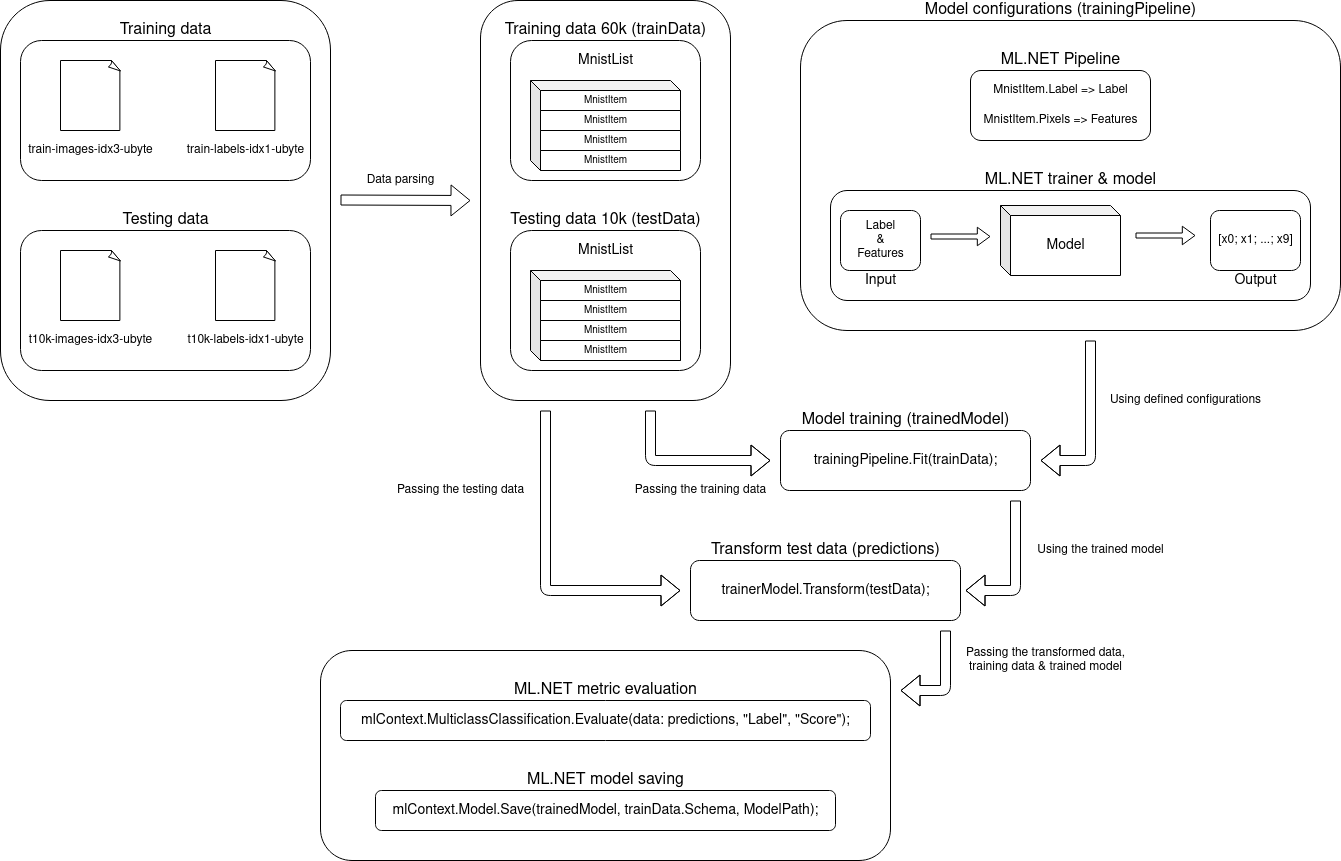
\includegraphics[width=15cm]{VPL-ML.png}
        \caption{ML modeļa trenēšanas diagramma}
        \label{ml:train}
    \end{figure}

    Projekta sākumā tika iegūti \texttt{MNIST} dati no "THE MNIST DATABASE". Tie ir 4 bināri faili
    un tos diagrammā var redzēt "Training data" un "Testing data" kvadrātos. Pēc datu iegūšanas tika
    izveidots datu parsēšanas funkcija, kas ielasa visus datus atmiņā un sadala tos pa klasēm
    \texttt{MnistList} un \texttt{MnistItem}. Šīm klasēm ir arī vizuāla reprezentācija diagrammā.
    Kad dati ir ielādēti atmiņā, tad tiek izveidots \texttt{ML.NET} "pipeline", kas ir kā konfigurācija
    priekš modeļa, kas tiks apmācīts. Visa konfigurācija ir redzama "Model configurations" kvadrātā. Šajā konfigurācijā
    tiek izveidots "pipeline", kas sasaista \texttt{Mnist} klašu mainīgos ar modeļa mainīgajiem.
    Tiek arī nodefinēta modeļa veids, kādi input dati būs un kādi output dati. Pēc datu ielasīšanas
    un modeļa nokofigurēšanas šis modelis tiek apmācīts. Lai šo modeli apmācītu, tiek izmantotas
    \texttt{ML.NET} iebūvētā metode: \texttt{.Fit()}. Šo funkcijju ir iespējams apskatīt "Model training"
    kvadrātā. Kad modelis ir apmācīts ir nepieciešams novērtēt cik labi šis modelis ir apmācīts, tapēc
    ir nepieciešams veikt transformācijas uz testa datiem tas ir redzams "Transform test data" kvadrātā,
    un tad, izmantojot šos pārveidotos testa datus, un \texttt{ML.NET} iebūvēto funkciju \texttt{.Evaluate()}
    tiek iegūtas modeļa rezultējošās metrikas. Pēdējais solis ir šo modeli saglabāt, kas arī tiek darīts
    izmantojot \texttt{ML.NET} iebūvēto funkciju \texttt{.Save()}.

    Rezultātā tika iegūts modelis, kuru metriku rezultāti ir redzami \ref{ml:metrics}~attēlā.

    \begin{figure}[H]
        \centering
        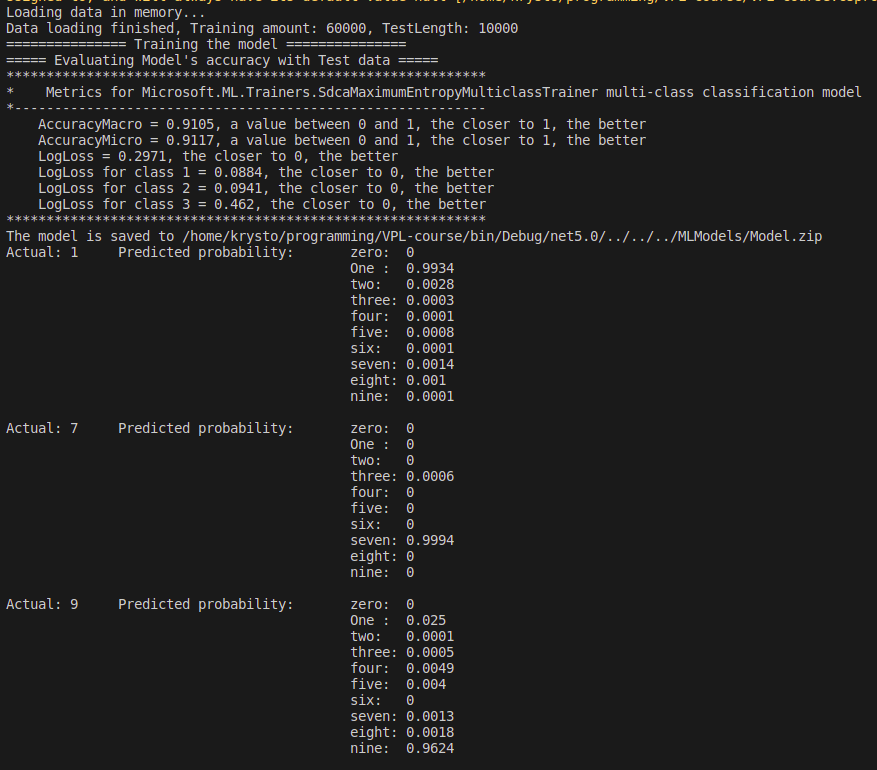
\includegraphics[width=13cm]{training-sc-v2.png}
        \caption{ML modeļa metriku rezultāti}
        \label{ml:metrics}
    \end{figure}

    Kad modelis bija izveidots, tad to bija nepieciešams implementēt tīmekļa aplikācijā. Tika izveidota
    \texttt{MnistClassificator} klase, kurā atrodas  metode \mintinline{csharp}{public float[] Analyze(byte[] image)}, kas tiek padota izveidotam modelim, kas atgriež
    virkni ar float vērtībām. Šīs vērtības reprezentē procentuālās vērtības ciparu klasēm.



    % Project results
    \section{Rezultāti}

Izstrādātās tīmekļa aplikācijas galvenie elementi ir redzami \ref{orig:lapasElementi} attēlā. Attēla kreisajā pusē ir redzams \texttt{svg} elements, uz kura lietotājs var zīmēt savu izvēlēto ciparu. Zem šī elementa ir pogas ar papildus funkcijām (\ref{orig:svgElementi} attēls). Uzspiežot pogu 'GUESS', zīmējums tiek saglabāts, analizēts un rezultāts ar zīmējuma samazināto versiju ir redzams attēla labajā pusē.

\begin{figure}[H]
    \centering
    \fbox{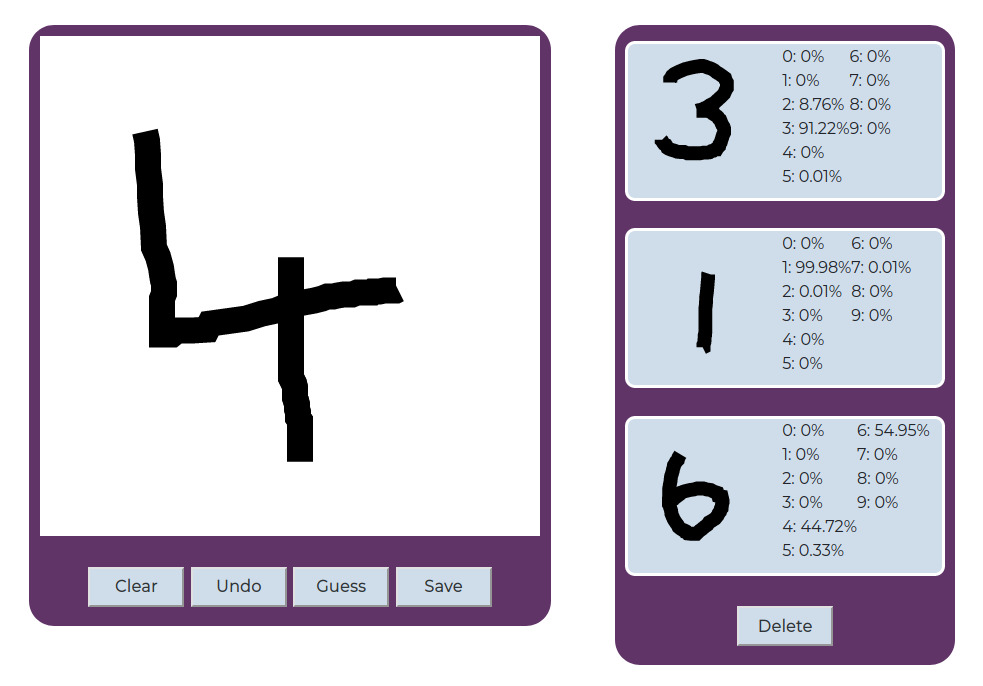
\includegraphics[width=120mm]{history.jpeg}}
    \caption{Tīmekļa aplikācijas elementi}
    \label{orig:lapasElementi}
\end{figure}

\begin{figure}[H]
    \centering
    \fbox{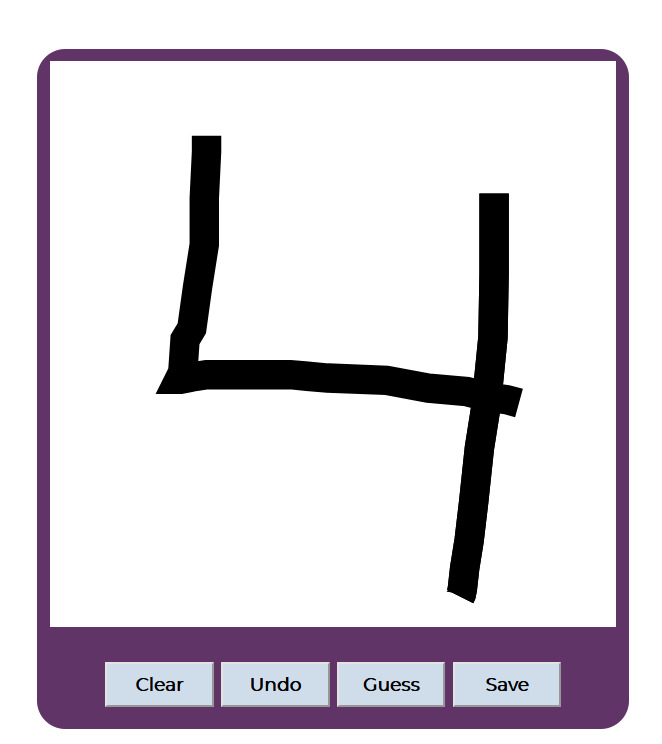
\includegraphics[width=120mm]{drawing.jpeg}}
    \caption{Galvenais svg elements un pogas}
    \label{orig:svgElementi}
\end{figure}

\par Zīmējumu vēstures skats ir redzams \ref{orig:selection} attēla labajā pusē. Sarakstam ir pielietota iespēja izvēlēties kādu no elementiem un izdzēst to no vēstures.

\begin{figure}[H]
    \centering
    \fbox{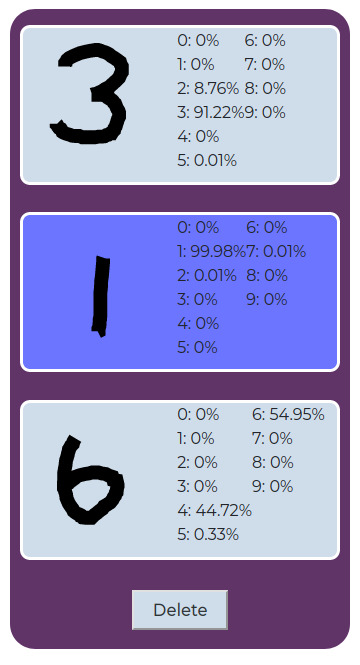
\includegraphics[width=120mm]{selection.jpeg}}
    \caption{Zīmējumu vēsture}
    \label{orig:selection}
\end{figure}

\par Viena no zīmējumam pievienotajām funckijām ir attēla saglabāšana. Šī funkcija nav izmantota nekur citur projektā. Tā nenes nekādu citu jēgu kā ļaut lietotājam lejupielādēt savu zīmējumu. Tā tiek pielietota, lietotājam nospiežot 'SAVE' pogu, kas redzama \ref{orig:svgElementi} attēlā. Ar šo pogu zīmējums tiek saglabāts kā png fails lietotāja datorā ar nosaukumu \textit{number.png}. \ref{orig:downloadedFile} attēlā redzams lejupielādētais zīmējums.
\begin{figure}[H]
    \centering
    \fbox{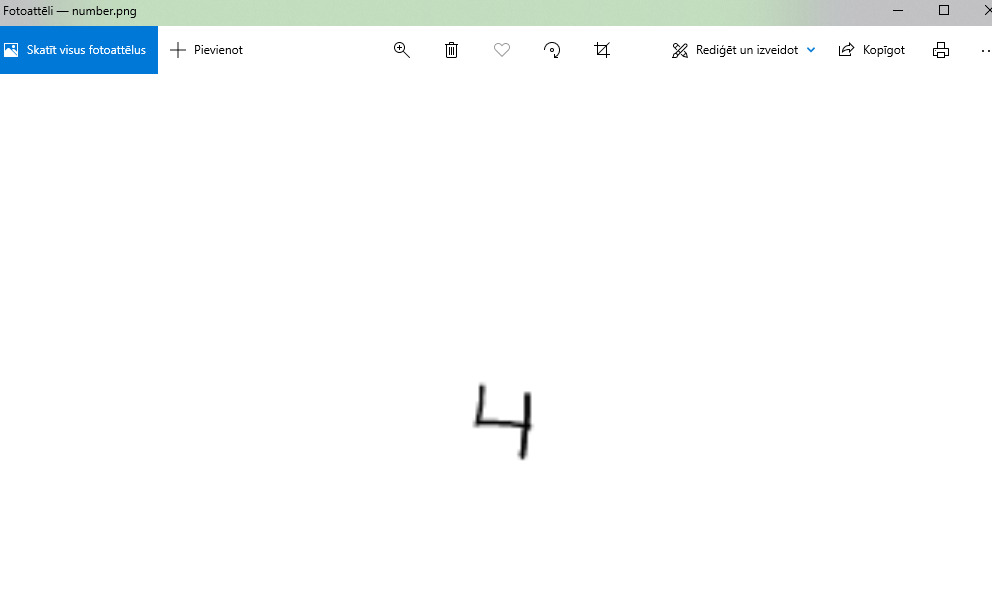
\includegraphics[width=120mm]{downloaded.jpeg}}
    \caption{Lejupielādētais attēls}
    \label{orig:downloadedFile}
\end{figure}



    % Conclusions after the project
    \section{Secinājumi}

    Darba koncepts likās samērā vienkāršs, un noteikti cilvēki, kas ar šādām tehnoloģijām ir jau
    ilgāku laiku strādājuši, šāda veida projekta izveide būtu vienkāršs process, bet tā kā darba autoriem
    šī bija pirmā pieredze, strādājot ar šādām tehnoloģijām, tad šī projekta izveide sagādāja dažādas
    grūtības. Projekta izveides procesā abi darba autori iemācījās daudz ko jaunu  un izsecināja
    dažādas lietas par \texttt{C\#} ekosistēmu.

    Galvenie secinājumi:
    \begin{itemize}
        \item \texttt{C\#} valodai un ietvariem ir labs atbalsts uz \texttt{Windows} operētājsistēmas;
        \item Strādāt ar \texttt{C\#} ietvariem un bibliotēkām ārpus \texttt{Windows} operētājsistēmas ir ļoti apgrūtinoši;
        \item Vispārīgi \texttt{C\#} mašīnmācīšanās ietvariem ir ļoti slikts uz \texttt{unix} bāzētām operētājsistēmām;
        \item \texttt{C\#} mašīnmācīšanās ietvari nenodrošina labu lietotāju pieredzi;
        \item Liela daļa \texttt{C\#} mašīnmācīšanās ietvaru ir vienkārši "\textit{api wrappers}" pāri python ietvariem kā, piemēram, \texttt{PyTorch} un \texttt{TensorFlow};
        \item \texttt{ML.NET} ir samērā spēcīgs rīks priekš mazu mašīnmācīšanās modeļu izveides;
        \item \texttt{ML.NET} ir tik ļoti abstrahēts, ka to ir ļoti grūti izmantot un izprast;
        \item Ir ļoti svarīgi izveidot pareizu modeļa arhitektūru, lai tas strādātu pareizi arī nestandarta apstākļos;
        \item \texttt{Python} un tā ietvari piedāvā labāku atbalstu priekš mašīnmācīšanās modeļu izveides nekā \texttt{C\#};
    \end{itemize}


    \par Tīmekļa aplikācijas izstrādei alternatīva bija izveidot \texttt{WPF} aplikāciju, ar kuru darba autori jau ir strādājuši kursa ietvaros. Izstrādājot projektu ar šo metodi, iespējams, ka darbs būtu paveikts ātrāk, būtu papildināts ar funkcionalitāti, papildus elementiem. Strādājot ar Blazor ietvaru, pagāja laiks, līdz tas tika iepazīts, tika saprasta tā funkcionalitāte un iespējas. Dažas no projektā izveidotajām funkcijām tika rakstītas \texttt{javascript} valodā, jo netika atrasta alternatīva \texttt{C\#} valodā.

    % References to used materials in the report
    \section{References}

    K


    % Appendix of extra materials
    \section{Pielikums}

    % Appendix for the created web page
    \subsection{Tīmekļa aplikācija}

\par Lai dinamiski varētu izveidot jaunus \texttt{polyline} elementus, tika izmantota \texttt{RenderFragment} \cite{render_fragment}  klase. Ar to var izveidot veidni priekš noteiktas komponentes. Koda daļā zem šī teksta var redzēt, kā šī klase tiek izmantota \texttt{svg} elementa izveidei, padodot tam jau esošu \texttt{polyline} sarakstu.

{
\setstretch{1.0}
\begin{minted}[]{csharp}
    private RenderFragment CreateSvg(List<RenderFragment> polylines) =>
    builder =>
    {
        int index = 0;
        builder.OpenElement(index++, "svg");
        builder.AddAttribute(index++, "viewBox", "0 0 100 100");
        builder.AddAttribute(index++, "preserveAspectRatio", "xMin meet");
        foreach (RenderFragment polyline in polylines)
        {
            builder.AddContent(index++, polyline);
        }
        builder.CloseElement();
    };
\end{minted}
}

\par Šī koda daļa atbild par \texttt{svg} pārveidi uz \texttt{Base64 string}, lai to varētu pārveidot uz \texttt{byte[]} \cite{from_base_64_to_string} formātu, kuru turpmāk izmanto faila saglabāšanai lietotāja datorā(kā \texttt{png}) un pārveidoto bitmap versiju mašīnmācīšanās algoritmam.
{
\setstretch{1.0}
\begin{minted}[]{csharp}
    protected async void SaveSvg(MouseEventArgs e)
    {
        await jsRuntime.InvokeAsync<string>("SaveSvg");
        hrefString = await jsRuntime.InvokeAsync<string>("getBase64");
        if(!String.IsNullOrEmpty(hrefString)){
            string toRemove = "data:image/png;base64,";
            string testString = hrefString.Replace(toRemove, "");
            bytes = Convert.FromBase64String(testString);
            saveFile(bytes);
        } else{
            SaveSvg(e);
        }
    }
\end{minted}
}

\par Lai uzzīmēto ciparu varētu attēlot zīmējumu vēstures skatā, ir nepieciešams to samazināt. Tādēļ tika izveidota šī funkcija \texttt{Scale}, kura samazina \texttt{polyline} elementa punktu vērtību par iedoto lielumu \textit{scale}.
{
\setstretch{1.0}
\begin{minted}[]{csharp}
    private string Scale(string pointsToRescale, double scale){
        string[] splittedPoints = pointsToRescale.Split(',');
        string newPoints = "";
        foreach(string point in splittedPoints)
        {
            if(Regex.Match(point, @"\d+\s\d+").Success)
            {
                string[] pair = point.Split(" ");
                Double x = Double.Parse(pair[0]);
                Double y = Double.Parse(pair[1]);
                x *= scale;
                y *= scale;
                newPoints += "," + x.ToString() + " " + y.ToString();
            }
            else
            {
                Double p = Double.Parse(point);
                p *= scale;
                newPoints+= p.ToString();
            }
        }
        return newPoints;
    }
\end{minted}
}

\par Lai pārveidotu \texttt{svg} failu uz \texttt{png} failu, tika izmantota \texttt{javascript} valoda un funkcija, kas tika pieminēta vienā no \texttt{stackoverflow} jautājuma atbildēm \cite{stackoverflow_answer}.

{
\setstretch{1.0}
\begin{minted}[]{javascript}
    function SaveSvg() {
        // Inline SVG element
        var mySVG = document.getElementById('mainSvg'),
        // Where to draw the result
        tgtImage = document.getElementById('mainCanvas'),
        // Not shown on page
        can = document.createElement('canvas'),
        ctx = can.getContext('2d'),
        // Not shown on page
        loader = new Image;
        loader.width = can.width = tgtImage.width;
        loader.height = can.height = tgtImage.height;
        let waitingForResult = true;
        let result = "";
        loader.onload = function(){
            ctx.drawImage( loader, 0, 0, loader.width, loader.height );
            tgtImage.src = can.toDataURL();
            result = tgtImage.src;
            waitingForResult = false;
        };
        var svgAsXML = (new XMLSerializer).serializeToString( mySVG );
        loader.src = 'data:image/svg+xml,' + encodeURIComponent( svgAsXML );
    }
\end{minted}
}

\par Zīmējot ciparu uz lapas \texttt{svg} elementa, ir paredzēts, ka, ja lietotājs ar peles kursoru izies no \texttt{svg} elementa zonas, zīmējums aptrūks. Tas tika pielietots, lai zīmejums neturpinātos neparedzētos gadījumos (lietotājs nav nospiedis peles taustiņu, lai turpinātu zīmējumu, bet šķērsojot elementu ar peles kursoru, zīmējums turpinās). Tāpēc nepieciešams izveidot funkciju, kas pārbauda, vai peles kursors ir ārpus nepieciešamā elementa. Tam tika izmantota \texttt{javascript} valoda, ar kuru varēja iegūt \texttt{svg} elementa atrašanāš vietu lapā un kursora koordinātas.
{
\setstretch{1.0}
\begin{minted}[]{javascript}
    function MouseIsOutOfSvg(e) {
        x=e.clientX;
        y=e.clientY;
        let svg = document.getElementById('mainSvg');
        return Number(x) < Number(svg.getBoundingClientRect().left)
        || Number(x) > Number(svg.getBoundingClientRect().right)
         || Number(y) < Number(svg.getBoundingClientRect().top)
         || Number(y) > Number(svg.getBoundingClientRect().bottom);
    }
\end{minted}
}


    % Appendix for the created ml model
    \subsection{Mašīnmācīšanās modelis}

    Šajā sadaļā tiks apskatītas tikai galvenās koda daļas, gan priekš
    modeļa apmācīšanas, gan modeļa implementācijas.

    Trenēšanas procesā bija nepieciešams \texttt{MNIST} datus sakārtotā formā uzglabāt atmiņā, tāpēc
    tika izveidotas 2 klases:

    \begin{itemize}
        \item \texttt{MnistList}
        \begin{itemize}
            \item \texttt{MnistItem[] Images}
        \end{itemize}
        \item \texttt{MnistItem}
        \begin{itemize}
            \item \texttt{float[] Pixels}
            \item \texttt{float Label}
        \end{itemize}
    \end{itemize}

    Sarakstā ir aprakstītas klases un šo klašu galvenie klašu mainīgie. Pēc šo klašu izveidošanas
    bija nepieciešams izveidot parsēšanu. Šī parsēšana notiek \texttt{MnistList} konstruktorā,
    un izplementāciju ir iespējams apskatīt sekojoši:

    \begin{minted}{csharp}
    public MnistList(string imagePath, string labelPath)
    {
        FileStream fsImages = new FileStream(
            imagePath, FileMode.Open
        ); // Images
        FileStream fsLabels = new FileStream(
            labelPath, FileMode.Open
        ); // Labels

        BinaryReader brImages = new BinaryReader(fsImages);
        BinaryReader brLabels = new BinaryReader(fsLabels);

        int magic1 = ReverseBytes(brImages.ReadInt32());
        int magic2 = ReverseBytes(brLabels.ReadInt32());

        // Tests if dataset magic numbers are correct
        if (magic1 != 2051)
            throw new Exception("Not a valid MNIST image data set");

        if (magic2 != 2049)
            throw new Exception("Not a valid MNIST label data set");

        int imgCount = ReverseBytes(brImages.ReadInt32());
        int labelCount = ReverseBytes(brLabels.ReadInt32());

        // Checks if for each image there is a label
        if (imgCount != labelCount)
            throw new Exception(
                "Number of items of the two files is not the same"
            );

        int imgRows = ReverseBytes(brImages.ReadInt32());
        int imgCols = ReverseBytes(brImages.ReadInt32());

        this.Length = imgCount;
        this.Rows = imgRows;
        this.Columns = imgCols;

        this.images = new MnistItem[this.Length];
        byte[][] item = new byte[Rows][];
        for (int i = 0; i < item.Length; i++)
            item[i] = new byte[Columns];

        for (int di = 0; di < this.Length; ++di)
        {
            for (int i = 0; i < item.Length; ++i)
            {
                for (int j = 0; j < item.Length; j++)
                {
                    byte b = brImages.ReadByte();
                    item[i][j] = b;
                }
            }
            byte label = brLabels.ReadByte();

            MnistItem newImg = new MnistItem(
                width: 28, height: 28, pixels: item, label: label
            );
            images[di] = newImg;
        }

        fsImages.Close();
        brImages.Close();
        fsLabels.Close();
        brLabels.Close();
    }
\end{minted}

    Par piemēru šīm klasēm tika ņemts \texttt{GitHub} piemērs \cite{paxbunPaxbunCntkMnistPractice2019}.
    \texttt{MNIST} dati ir binārie dati un to pikseļu vērtības ir intervālā no 0 līdz 255,
    bet, ja modelim tiks doti normalizēti dati, kas ir vērtībās no 0 līdz 1, tad tas
    apmācīts labāk. Tāpēc \texttt{MnistItem} klases konstruktorā šie dati tiek
    normalizēti.

    \begin{minted}{csharp}
    public MnistItem(int width, int height, byte[][] pixels, byte label)
    {
        this.Width = width;
        this.Height = height;
        this.Label = label;

        this.Pixels = new float[height*width];

        int counter = 0;
        for (int i = 0; i < height; ++i)
        {
            for (int j = 0; j < width; ++j)
            {
                this.Pixels[counter] = ((float)pixels[i][j]) / byte.MaxValue;
                counter += 1;
            }
        }
    }
\end{minted}

    Pēc datu ielasīšanas ir nepieciešams apmācīt modeli. Priekš tā tika izveidota funkcija, tika ņemts jau eksistējošs piemērs no \texttt{ML.NET} \texttt{GitHub}
    repozitorija \cite{DotnetMachinelearningsamples2021}. Dotajā piemērā izmantotā datu kopa
    neatbilda īstajai \texttt{MNIST} datu kopai, bet gan daudz mazākai datu kopai, tāpēc šo piemēru bija
    jāpārveido, lai tas darbotos ar nepieciešamo \texttt{MNIST} datu kopu. \cite{MNISTHandwrittenDigit}

    \begin{minted}{csharp}
    public static void Train(
        MLContext mlContext, MnistList trainingData, MnistList testingData
    )
    {
        try
        {
            // 1: Data loaded into mlContext
            var trainData = mlContext.Data.LoadFromEnumerable<MnistItem>(
                trainingData.images
            );
            var testData = mlContext.Data.LoadFromEnumerable<MnistItem>(
                testingData.images
            );

            // 2: Context data process configuration with pipeline
            // data transformations
            var dataProcessPipeline = mlContext.Transforms.
                Conversion.MapValueToKey(
                    "Label", "Label",
                    keyOrdinality: ValueToKeyMappingEstimator.
                        KeyOrdinality.ByValue
                ).
                Append(
                    mlContext.Transforms.Concatenate(
                        "Features", nameof(MnistItem.Pixels)
                    ).AppendCacheCheckpoint(mlContext)
                );

            // 3: Set the training algorithm, then create and config
            // the modelBuilder
            var trainer = mlContext.MulticlassClassification.
                Trainers.SdcaMaximumEntropy(
                    labelColumnName: "Label", featureColumnName: "Features"
                );
            var trainingPipeline = dataProcessPipeline.Append(trainer);

            // 4: Train the model fitting to the DataSet
            Console.WriteLine(
                "=============== Training the model ==============="
            );
            ITransformer trainedModel = trainingPipeline.Fit(trainData);

            Console.WriteLine(
                "===== Evaluating Model's accuracy with Test data ====="
            );
            var predictions = trainedModel.Transform(testData);
            var metrics = mlContext.
                MulticlassClassification.Evaluate(
                    data: predictions, labelColumnName: "Label",
                    scoreColumnName: "Score"
                );

            Common.ConsoleHelper.PrintMultiClassClassificationMetrics(
                trainer.ToString(), metrics
            );

            // If there is already a trained model then this will
            // override that model
            mlContext.Model.Save(trainedModel, trainData.Schema, ModelPath);

            Console.WriteLine("The model is saved to {0}", ModelPath);
        }
        catch (Exception ex)
        {
            Console.WriteLine(ex.ToString());
        }
    }
\end{minted}

    Rezultātā tika izveidots modelis, kuru bija nepieciešams implementēt tīmekļa aplikācijā.
    Tika izveidota klase \texttt{MnistClassificator} ar metodi, kura saņem masīvu ar pikseļu vērtībām un
    atgriež masīvu ar float vērtībām, kur katrs elements
    atbilst kādai no ciparu klasēm.

    \begin{minted}{csharp}
    /*
    Input parameters
    ----------------
    image: 784 array, each value is between 0 and 255 (white - black)
    */
    public float[] Analyze(byte[] image)
    {
        if (image.Length != 784)
            throw new Exception("Image length is not 784.");

        MnistItem imageObject = new MnistItem(
            length: image.Length, pixels: image
        );

        MLContext mlContext = new MLContext();
        var predEngine = mlContext.Model.
            CreatePredictionEngine<MnistItem, MnistOutPutData>(
                this.trainedModel
            );

        var output = predEngine.Predict(imageObject);

        return output.Score;
    }
\end{minted}

    Lai ielasītu modeli atmiņā un to varētu izmantot tiek izmantota \texttt{ML.NET} funkcija:
    \mintinline{csharp}{this.trainedModel = mlContext.Model.Load(ModelPath, out var modelInputSchema);}




\end{document}
